\chapter{RESULTADOS EXPERIMENTAIS}
\label{chap:proposta_experimental}

Este capítulo traz informações relacionadas com as ferramentas utilizadas no experimento, como linguagem, biblioteca, entre outros. Informações sobre o conjunto de dados \gls{ACDC} e SunnyBrook, o consumo de ambos no modelo base e nas versões adaptadas. Por fim, são apresentados resultados experimentais com o conjunto de dados \gls{ACDC}. 

%--------------------------------------------------------
\section{Materiais} 
\label{sec:cap5_materiais}

Esta seção visa trazer informações sobre tanto o \textit{hardware} quanto o \textit{software}, como também as principais bibliotecas utilizadas e suas versões nos experimentos para fins de reprodução. A Tabela \ref{tab:hardware_software} estrutura estas informações. Outra ferramenta utilizada no registro dos experimentos foi o CometML\footnote{https://www.comet.com}. Esta auxiliar armazenar informações como erro no processamento do lote, acurácia de do conjuntos de validação, entre outros no treino de modelo de redes neurais.
\newline

\begin{table}[hbtp]
    \centering
    \renewcommand{\arraystretch}{1} % default é 1 
    % \begin{tabular}{|>{\centering\arraybackslash}p{2cm}|p{12cm}|}
    \begin{tabular}{|c|c|}
    \hline 
       \textbf{Item} & \textbf{Descrição}\\
    \hline 
       Computador & \textit{Macbook M1 Pro}  \\
    \hline 
       Memória & 16gb  \\
    \hline 
       Versão \textit{Python} & 3.11.0  \\
    \hline 
       Versão \textit{pyradiomics} & 3.0.1 \\
    \hline 
       Versão \textit{torch} & 2.2.1 \\
    \hline 
       Versão \textit{torchvision} & 0.17.1 \\
    \hline 
       Versão \textit{numpy} & 1.26.4 \\
    \hline 
       Versão \textit{scikit-learn} & 1.4.1.post1 \\
    \hline 
       Versão \textit{comet-ml} & 3.47.4 \\
    \hline 
    \end{tabular} 
    \caption{Fonte: Autor}
    \label{tab:hardware_software}
\end{table}

%--------------------------------------------------------
\section{Conjunto de Dados} 
\label{subsec:cap5_dataset}

Este trabalho visa realizar os experimentos em duas bases distintas com imagens de \gls{RMC}, informações a cerca do paciente e rótulos que indicam presença ou não de cardiomiopatia. Testes iniciais foram feitos no conjunto de dados \gls{ACDC}. O \gls{ACDC} possui $30$ casos de \gls{CMH}, $30$ casos de \gls{CMD} e $90$ casos normais. Da base \gls{ACDC} se pretende utilizar apenas as fatias da fase diastólica. O segundo conjunto de dados é o SunnyBrook, possuindo imagens na fase diastólica contendo as classes NOR(normal) e HIP(hipertrofia do ventrículo esquerdo)três classes de interesse previamente mencionadas. 

O modo de operação será o mesmo para ambos os conjuntos de dados com exceção do pré-processamento dado o fato de ambos os conjuntos serem diferentes quanto aos dados.

%--------------------------------------------------------
\subsection{Experimentos Modelo Base}
\label{subsec:cap5_experimentos_base}

Uma prova de conceito foi aplicada ao conjunto de dados \gls{ACDC} utilizando o modelo de linha de base para uma primeira avaliação de referência. O modelo base foi implementado seguindo o artigo e sua implementação é conferida na Figura \ref{fig:fig008}. O conjunto de dados para treino é composto por $100$ exames de pacientes, coletando apenas as fatias das imagens da fase diastólica. Características de primeira ordem e \gls{GLCM} são extraídas, utilizando a blbioteca \textit{PyRadiomics}, resultando em $\RadiomicFeatures$ valores que compõem as características radiômicas. Para extração das características profundas, foi utilizado uma rede \textit{ResNet50} congelada sem sua última camada linear, responsável pela classificação originalmente de $1000$ classes oriundas do conjunto de dados \textit{ImageNet}, obtendo como resultado final um vetor com $\DeepFeatures$ valores características profundas.

O \textit{F-Test} é utilizado como um seletor de características inicial, aplicado tanto nas características radiômicas e profundas, com um total de $\text{EMBED}_{size}$ igual a $12$  no modelo base. As características resultantes do \textit{F-Test}, agora com tamanhos agora iguais, são concatenadas e enviadas ao módulo de autoatenção e os resultados armazenados.

Neste experimento foi treinado o modelo utilizando, como função objetivo a entropia cruzada binária, taxa de aprendizado de $\LR$, otimizador \textit{Adam}, tamanho de lote $\Batch$ e o treinamento se deu com aproximadamente $\Epochs$ épocas, onde verificou que o erro se torna estável em tempo de treinamento. Também foi empregada a estratégia de aleatorizar as entradas do modelo e descartar o último lote caso ele seja menor que os demais lotes processados. Com a saída do modelo é aplicada a função sigmoide, Equação. \ref{eq:sigmoide}, função esta que limita os valores de sua entrada entre 0 e 1. Para fins de classificação, foi considerado valores maiores que $0,5$ são considerados com \gls{CMH} e menores ou iguais a $0,5$ são considerados normais.

\begin{equation}
\textit{sigmoide}(x) = \frac{1}{1 + e^{-x}}
\label{eq:sigmoide}
\end{equation}

% --------------------------------------------------------
\subsection{Experimentos Modelos Adaptados}
\label{subsec:cap5_experimentos_adaptados}

Os modelos adaptados refletem os experimentos desmembrados do modelo base, adaptações estas com a finalidade de verificar se mudanças, seja nos hiperparâmetros, seja em partes da arquitetura, podem trazer resultados promissores em relação aos resultados base.

As mudanças podem ser elencadas em: mudanças do $\text{EMBED}_{size}$ onde se foi testado os valores $[24, 48, 64]$ na tentativa de preservar mais informações originais. Na versão adaptada também há o consumo das respectivas máscaras que são futuramente concatenadas as características radiômicas e profundas. A concatenação é feita de forma diferente também, assumindo por exemplo $\text{EMBED}_{size} = 12$, na versão original temos como resultado $1\times24$ porém na versão adaptada essa concatenação é feita na primeira dimensão, resultando neste exemplo em $2\times12$. Isto se dá pois é apresentado um novo bloco ao modelo original o bloco convolucional, composto de convolução e blocos \gls{SE}. A parte restante da arquitetura segue de acordo com a original, exceto que também podemos variar $N$ vezes o bloco de autoatenção, ou seja, sua saída volta sendo sua entrada $N$ vezes e este valor de $N$ também pode ser imaginado como um dos hiperparâmetros do experimento.

% Posso elencar novamente de forma sucinta os hiperparamentros aqui: EMBED_SIZE, N attention blocks, imagems de mascara e nova forma de concatenar. 


%--------------------------------------------------------
% \section{Cronograma}
% \label{sec:cronograma}

% O cronograma proposto das atividades segue na Figura \ref{fig:fig014}. Os itens em azul são atividades concluídas como: disciplinas, revisão bibliográfica, refinamento do tema, testes iniciais, etc. Itens em rosa são atividades em andamento como: implementação de modelos de comparação e escrita da dissertação. Atividades em amarelo são atividades planejadas como: análise de resultados, escrita da dissertação e escrita de artigos.

% \begin{figure}[htbp]
%     \centering
%     \caption{Cronograma planejado}
%     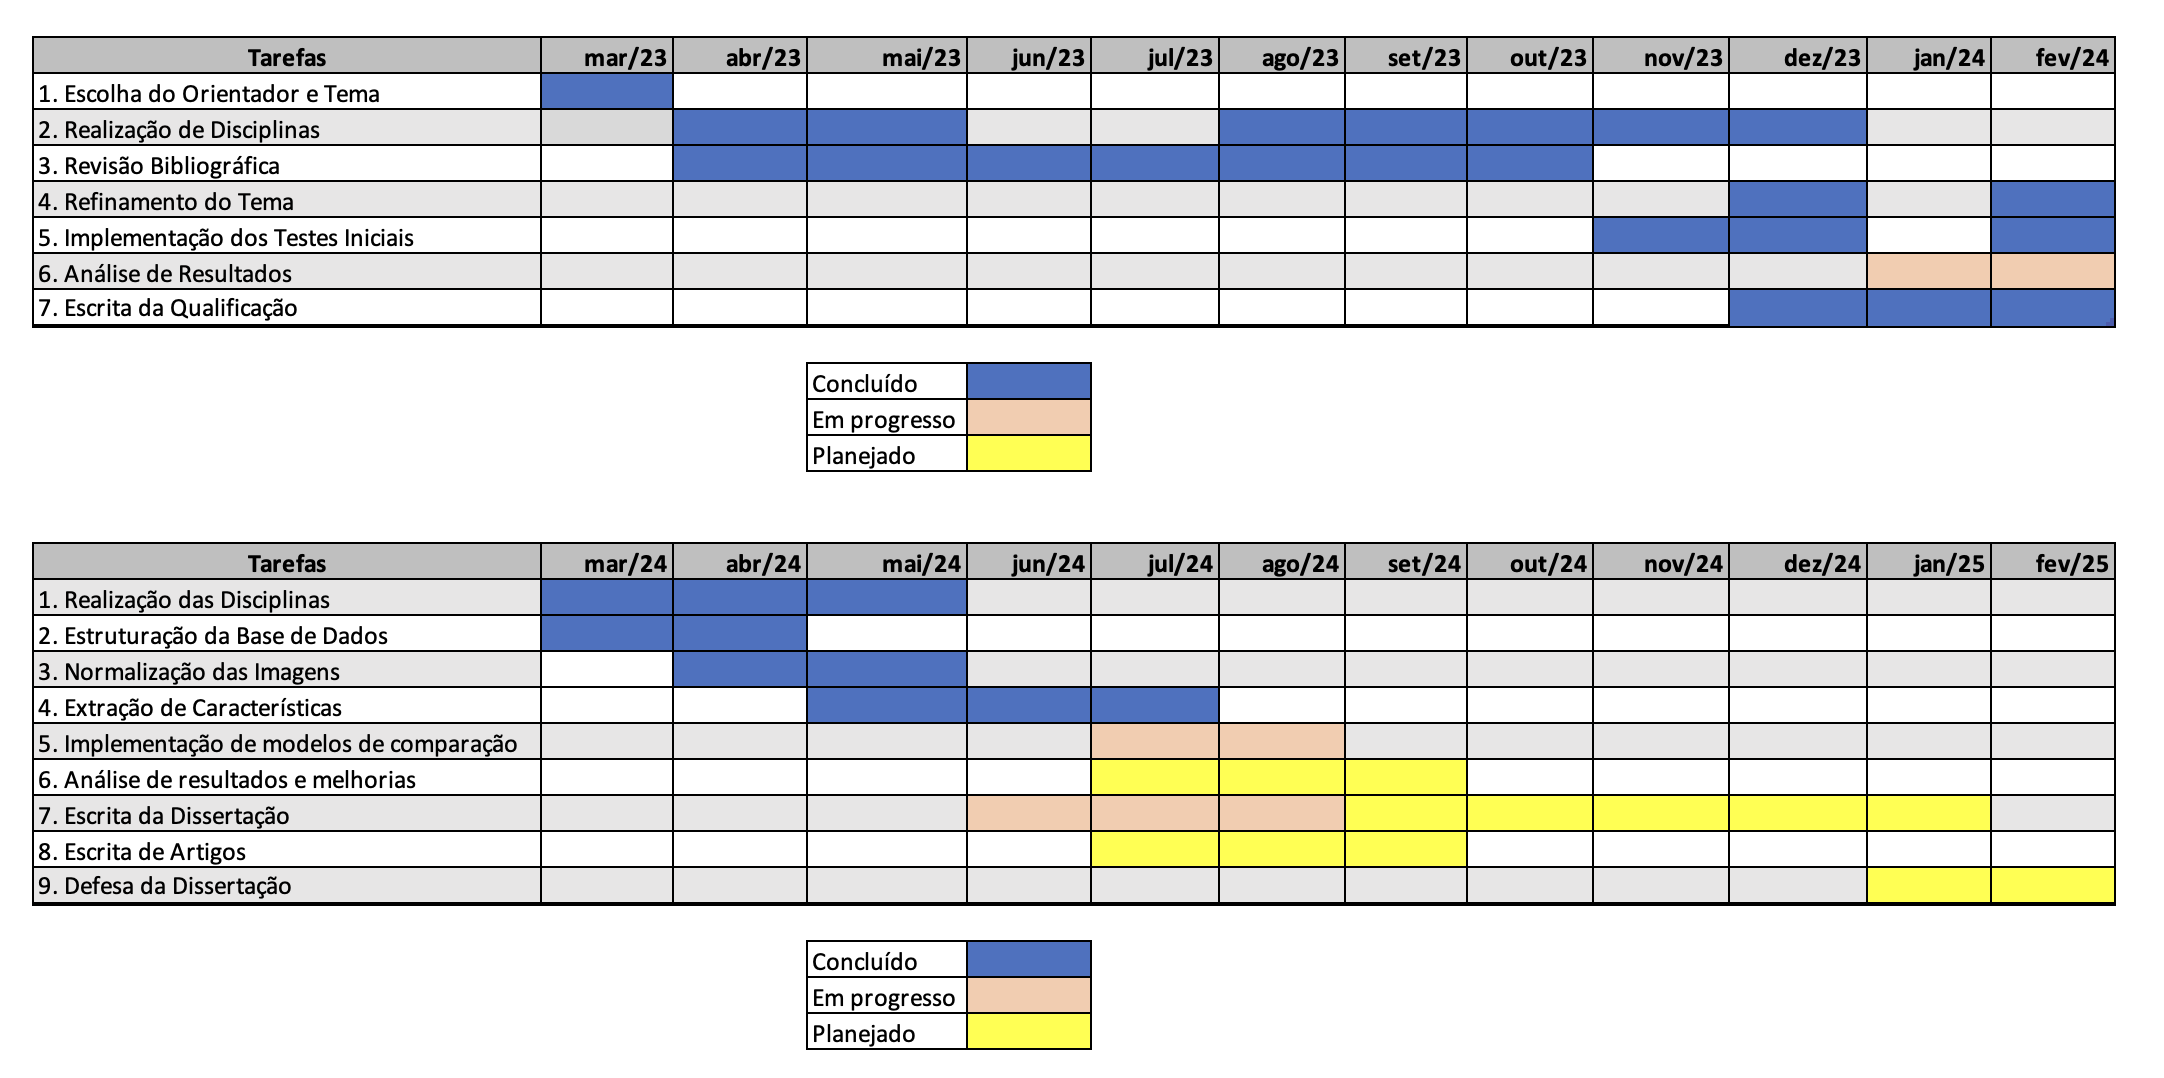
\includegraphics[width=1\textwidth]{figures/fig014.png}
%     \caption*{Fonte: Autor}
%     \label{fig:fig014}
% \end{figure}
